\chapter{Background}\label{chapter:background}

To properly understand FLOps as a whole and why it combines different techniques, it is necessary to analyze them individually.
This analysis includes critical background knowledge of their benefits and downsides.
Only afterward does it make sense to discuss how FLOps merges them to create something new.

This background chapter provides a general overview of each sector and discusses aspects necessary for FLOps in greater detail.
The first section explores the field of federated learning.
FL is the core task at hand that FLOps aims to optimize.
A thorough understanding of this discipline is required to determine its shortcomings.
The following section discusses established best practices from DevOps and MLOps to improve upon these weaknesses.
Techniques like automation and CI/CD require infrastructure and resources.
Orchestration enables provisioning, management, and deployment of such infrastructure and resources.
Its section reviews orchestration technologies and provides a short overview of Oakestra as the chosen platform for FLOps.
In the final background section, a couple of existing works resembling FLOps are examined and compared.


\section{Federated Learning}\label{section:federated_learning}

This section contains necessary background information and context regarding FL.
The first subsection covers fundamental FL building blocks and terminologies.
The next subsection explains vital supplementary FL concepts.
Oakestra orchestrates FLOps.
It uses an unconventional three-tiered structure that allows support for geographical clusters \cite{paper:oakestra_usenix}.
This structure opens up unique opportunities for FL applications.
More advanced FL architectures are necessary to benefit from these opportunities.
The following subsection discusses these architectures.
These three subsections build a solid FL understanding.
A great summary and source of information for deeper insights into the field of FL can be found in \cite{book:fl}.


\subsection{FL Basics}

\begin{figure}[h]
    \centering
    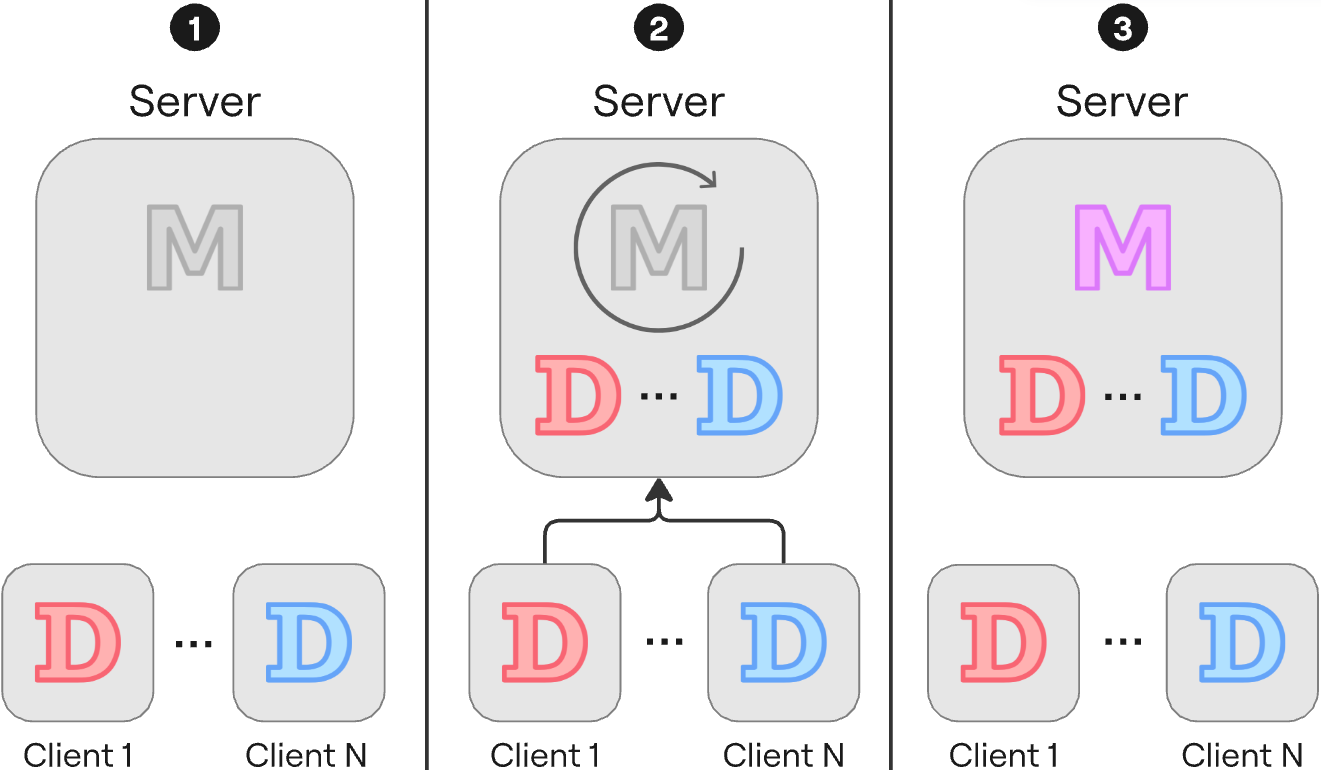
\includegraphics[width=0.9\textwidth]{classic_ml_training.png}
    \caption{Centralized ML Model Training}
    \label{fig:classic_ml_training}
\end{figure}
Figure \ref{fig:classic_ml_training} depicts the classic centralized ML model training process.
Starting from (1), where clients have their data (D) and the server hosts the untrained (gray) ML model (M).
In (2), the clients send their data to the server.
The server can now train the model using data from the clients.
(3) depicts the final state after training.
(The pink/purple model color symbolizes that different data sources have been used during training.)
The client data remains on the server and is exposed to potential exploitation.
As discussed in the introductory chapter, this centralized approach often leads to privacy breaches.

FL was introduced to use sensitive data on client devices for training ML models while keeping that data private.
Thus, FL complies with laws and regulations.
Many different algorithms and strategies exist for FL.
The following example focuses on the widely used base-case/classic FL algorithm FederatedAveraging (FedAvg) \cite{paper:original_fl}.

\begin{figure}%[h]
    \centering
    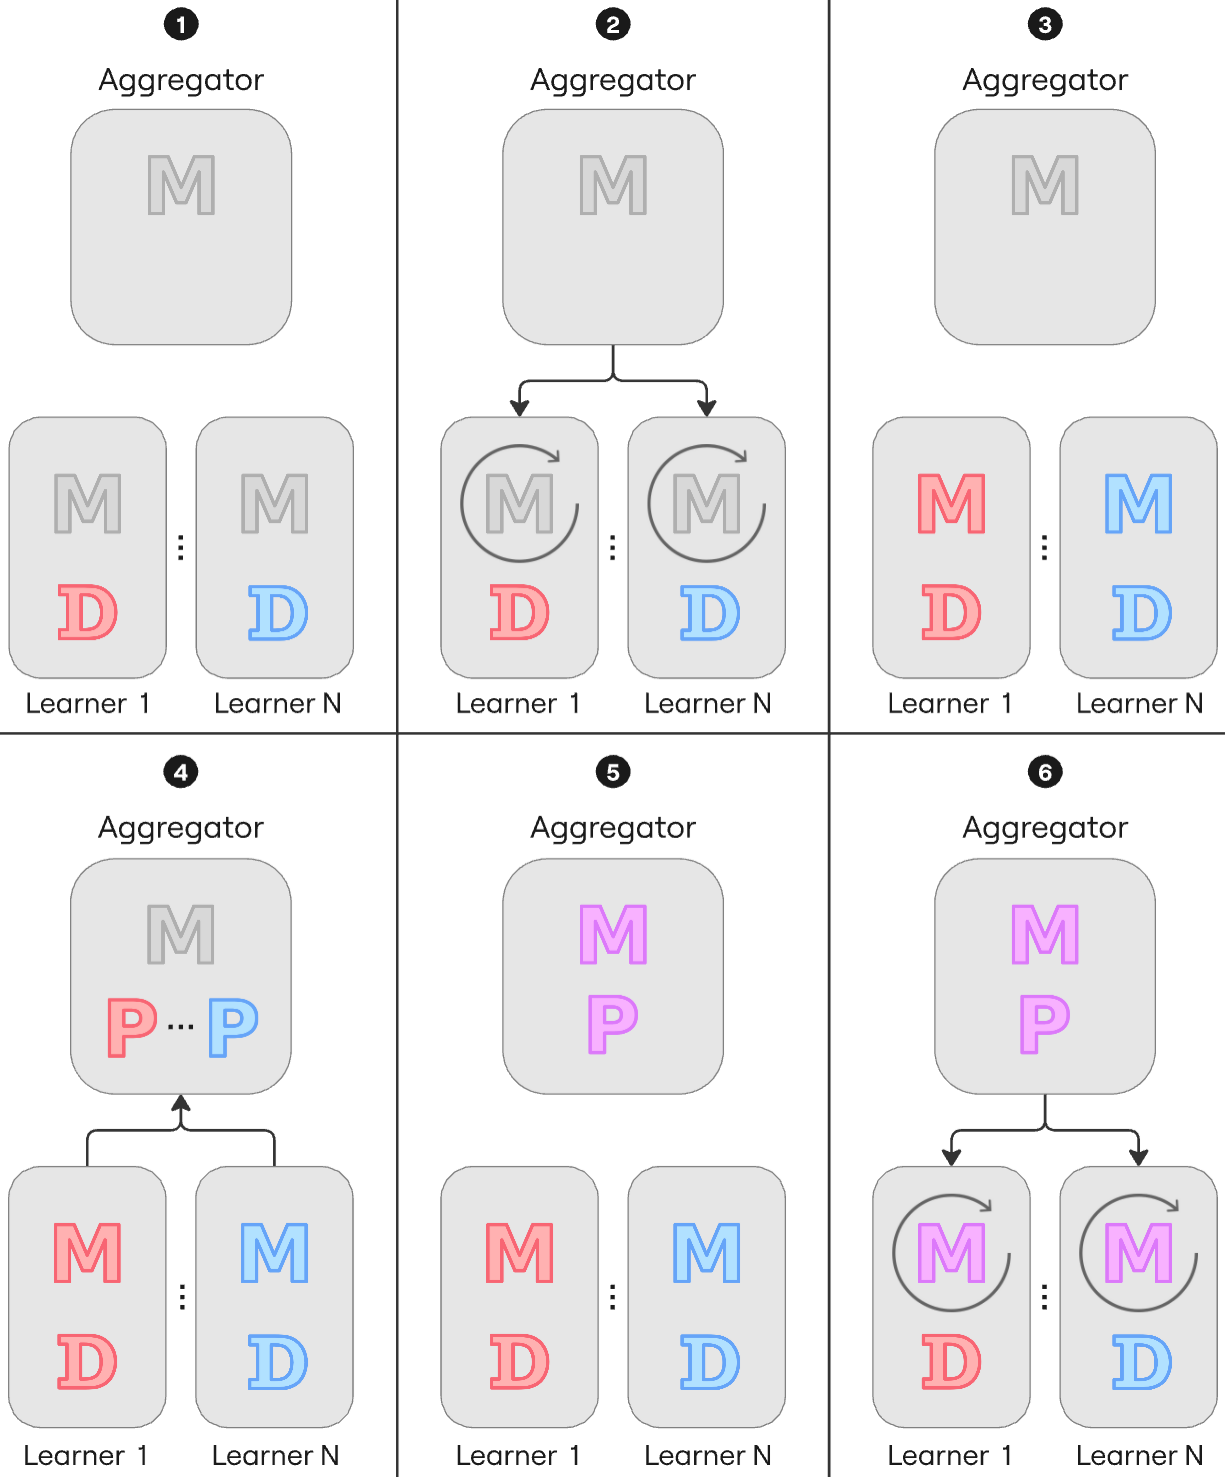
\includegraphics[width=\textwidth]{basic_fl_intro.png}
    \caption{Basic Federated Learning}
    \label{fig:basic_fl_intro}
\end{figure}
Figure \ref{fig:basic_fl_intro} shows the basic FL training loop.
The number of learners can vary.
The first differences are the component names.
In FL, the server is frequently called an \textbf{aggregator}, and it coordinates the FL processes.
Clients are called \textbf{learners}.
Using the terms server and clients in FL is still common
\footnote{
FLOps uses various components, including non-FL servers and clients.
Therefore, this work prefers aggregators and learners because they highlight FL components and help with comprehension.
}.
Another difference is that all components must know and possess the ML model locally.
They also need to set up their environment for training properly.

As a reminder, one can split up ML models into two parts.
One part is (usually) a static lightweight model architecture.
It includes layer specification (in DNNs), training configuration, and hyperparameters like learning step sizes, loss, and activation functions.
Model weights and biases are the dynamic components of an ML model.
A model without them is not useful because weights and biases are what get trained.
They allow the model to fulfill its intended use, such as prediction, inference, or generation tasks.
These weights and biases are the major contributors to a trained model's overall size (space utilization).
Model architecture is static in classic ML/FL.
Thus, FL components can transmit and share weights and biases instead of the entire trained model.
This work calls model relevant data sent between the learners and aggregators (model) \textbf{parameters} and depicts it with (P).

The concrete classic FL steps are as follows.
Initially, at (1), all models are untrained.
At (2), the aggregator starts the first FL training cycle by telling the learners to start their local training.
The local training rounds (epochs) are completed at (3).
(The 'M's are now colored.)
In (4), the learners have extracted their model parameters and sent them to the aggregator.
The aggregator now has access to these parameters but not the sensitive data used to train them.
That is how FL can profit from sensitive data while maintaining its privacy.
Possible attack vectors still exist.
They expose sensitive client information by abusing this parameter-based aggregation process.

In (5), the server aggregates these collected parameters into new global parameters.
This aggregation process is also called model fusion \cite{book:fl}.
The aggregator applies these global parameters to its model instance.
Learners can be heterogeneous and possess varying amounts of data.
Therefore, some learner updates might be more impactful than others.
To respect this circumstance, learners typically also send the number of data samples they used for training to the aggregator.
That way, the aggregator can prioritize its received updates proportionally.
Otherwise, in classic FL aggregation, the mean of the parameters is used for the global model.
The result is a \textbf{global model} that was trained for one FL cycle.

In (6), the aggregator sends its global parameters back to the learners.
The learners apply these parameters to their local model instance to make it identical to the aggregator's global model.
By doing this, learners discard their locally trained parameters.
The FL training loop could terminate, and the learners or servers could use their global model copy for inference.
Otherwise, as depicted in (6), another FL training cycle begins.
There can be arbitrarily many FL cycles, similar to conventional training rounds in classic ML.
FL training eventually terminates due to time/resource constraints or a failure to reach a satisfying performance.
If not terminated, the accuracy and loss will worsen due to overfitting, assuming the available training data is finite and unchanging.

\subsection{Supplementary FL Concepts}

This subsection explores essential supplementary FL concepts to understand the field better.

\subsubsection{FL compared to Distributed Learning}

FL and Distributed Learning (DL) are two related disciplines.
Instead of executing complex ML computations on a centralized resource-rich monolithic machine or data center, both techniques
distribute this computational load among multiple more resource-constrained machines that train individually.
These approaches increase convergence times and avoid needing expensive singular devices with sufficient resources.
After distributively training models, a server aggregates a global model.

The differences between both mechanisms are the following.
FL can use highly heterogeneous non-IID training data.
Quantity and distribution can vary significantly between learners.
FL can handle this varied data without having access to explicit information about their properties before or during training.
FL only utilizes the data that learners offer.
FL can work with a fluctuating number of learners that only participate in a small fraction of training rounds.
This dynamicity leads FL to handle various unique challenges, such as handling errors caused by crashed, failed, or disconnected learners during training.
On the contrary, DL initializes with total centralized access and control to all data before distributing it among its fixed and predefined clients \cite{book:fl}.
DL does not support FL's privacy concerns because it has complete oversight and control of all data.


\subsubsection{FL Variety}
FL is a diverse discipline with various possible applications and use cases.
Most FL work focuses on end-user/edge/IoT devices.
FL is not exclusive to these environments and can work in conventional cloud environments.
As discussed in the first subsection, FL can train DNNs.
FL can also apply to classic ML models, such as linear models (logistic regression, classification, and more) or decision trees for explainable classifications.
FL also supports horizontal, vertical, and split learning.
This work omits discussing these techniques to avoid bloat.
More information about these and other methods is available in \cite{book:fl}.
Plenty of FL optimizations exist for each ML variant, such as custom algorithms and strategies.

Personalization can help if the global model is too general and does not satisfy a learner's individual needs.
Different personalized FL (PFL) approaches exist.
Some take the final trained global model and further train it on local data (fine-tuning).
Other techniques train two local models concurrently.
The first model gets shared and updated with the global parameters.
The second one stays isolated and only gets influenced by local data.
A mixture between the global and purely local model can be used for inference.
PFL is a deep and growing subfield of FL \cite{book:fl,hpfl_over_massive_mobile_edge_computing_networks, paper:adaptive_exper_models_for_pfl}.

\subsubsection{FL Security \& Privacy}
The field of FL prioritizes security and privacy because protecting those was the key motivation for FL's creation.
FL should use secure and authenticated communication channels to prevent messages from being intercepted, read, or impersonated by a man-in-the-middle adversary.
One should ensure that learners and aggregators are the only actors with access to those messages and can decipher them.
A variety of FL adversaries and threats exist.
Fortunately, there exists a growing array of defenses against those threats.
It is crucial to pick and combine these defenses wisely based on the use case and environment.
Two prominent techniques to protect against threats are differential privacy and secure aggregation. \cite{book:fl}

We omit further detailed discussions because FLOps does not focus on privacy or security.

\subsection{FL Architectures}

FL comes in two broad structural categories.
Cross-silo or enterprise FL gets used in large data centers or multinational companies.
Each learner represents a single institution or participating group.
There are only around ten to a few dozen learners involved.
Cross-silo FL considers the identity of the parties for training and verification.
Generally, every individual local update from every learner at every training round is significant.
Fallouts and failures of individual learners are serious.
Cross-device FL can include hundreds or millions of devices, primarily edge/IoT devices.
Due to this great pool of learners, only a subset typically trains per round.
The identities of the participating learners are usually unimportant.
Due to the nature of these devices and their environments, cross-device FL needs to manage special challenges.
Challenges include non-IID data, heterogeneous device hardware, different network conditions, learner outages, or stragglers.
Various techniques exist to navigate these challenging conditions, including specialized algorithms for aggregation or learner selection.
These strategies can consider bias, availability, resources, and battery life.
\vspace{2mm}
\newline\textbf{From now on, when we mention FL in this work, we mean cross-device FL because FLOps focuses on cross-device workloads.}
\vspace{5mm}
\newline
Different FL architectures exist to support large-scale FL environments.
FLOps wants to benefit from the unique three-tiered Oakestra \cite{paper:oakestra_usenix} architecture.
Such a scenario has two main challenges.
The first challenge is managing a massive number of connections and aggregations.
The second one is reducing the negative impact of straggling learner updates.
The problem with using a single aggregator, as seen in \ref{fig:basic_fl_intro}, is that this single aggregator becomes a communication bottleneck.
Additionally, per-round training latency is limited by the slowest participating learner.
Thus, stragglers turn into another bottleneck.
The following is an overview of prominent FL architectures.

\subsubsection{Clustered FL}

\begin{figure}[b]
    \centering
    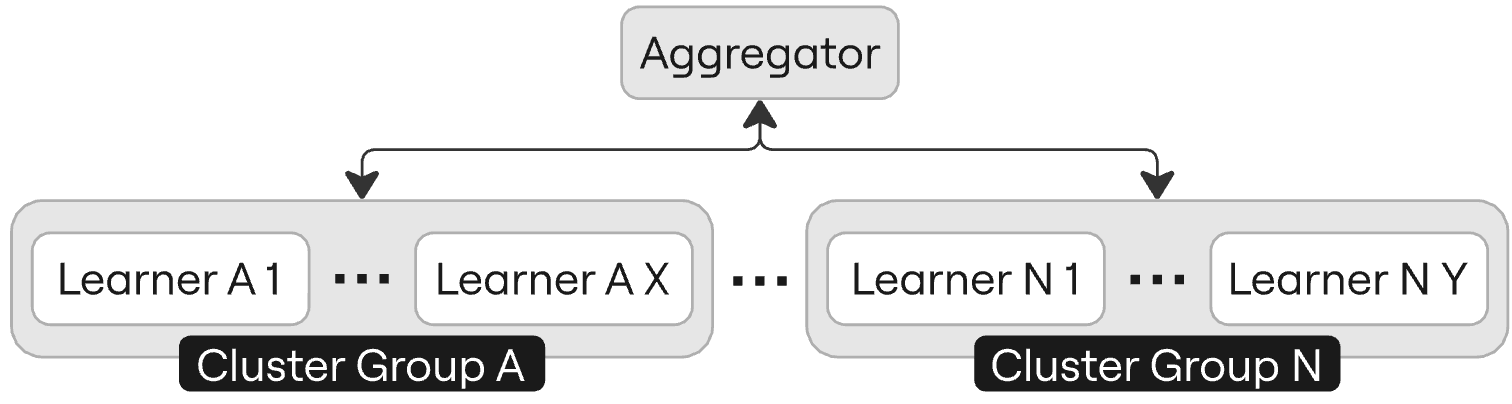
\includegraphics[width=\textwidth]{clustered_fl.png}
    \caption{Clustered FL Architecture}
    \label{fig:clustered_fl}
\end{figure}
Figure \ref{fig:clustered_fl} shows the Clustered FL (CFL) architecture that groups similar learners into clusters.
CFL can form clusters based on local data distribution, training latency, available hardware, or geographical location.
The issue of the singular aggregator as a bottleneck persists.
The main challenge for CFL is choosing a suitable clustering strategy and criteria for the concrete use case.
If the criteria are biased, updates from preferred clusters might be heavily favored, resulting in a biased global model with bad generalization.
Another task is to properly profile the nodes to match them to the correct cluster.
The entire cluster suffers if a slow outlier is present in a cluster.
Node properties can vary over time, so cluster membership has to be dynamic.
Too intrusive profiling can lead to compromised privacy.
The benefits of CFL are its ease of implementation, familiar architecture to classic FL, and flexibility to tune clustering/selection dynamically.
CFL can be combined with other architectures.
A downside of CFL is that a proper clustering strategy is use-case-dependent and challenging to optimize.
CFL does not really solve scalability issues on its own.
Its clustering overhead becomes critical with larger numbers of nodes.
\cite{
    paper:cluster_based_secure_aggregation_for_fl,
    paper:fedat_high_performance_communication_efficient_fl_with_asynch_tiers,
    book:fl,paper:decentralized_edge_intelligence_dynamic_resource_allocation_framework_hfl}

\subsubsection{Hierarchical FL}
\begin{figure}[b]
    \centering
    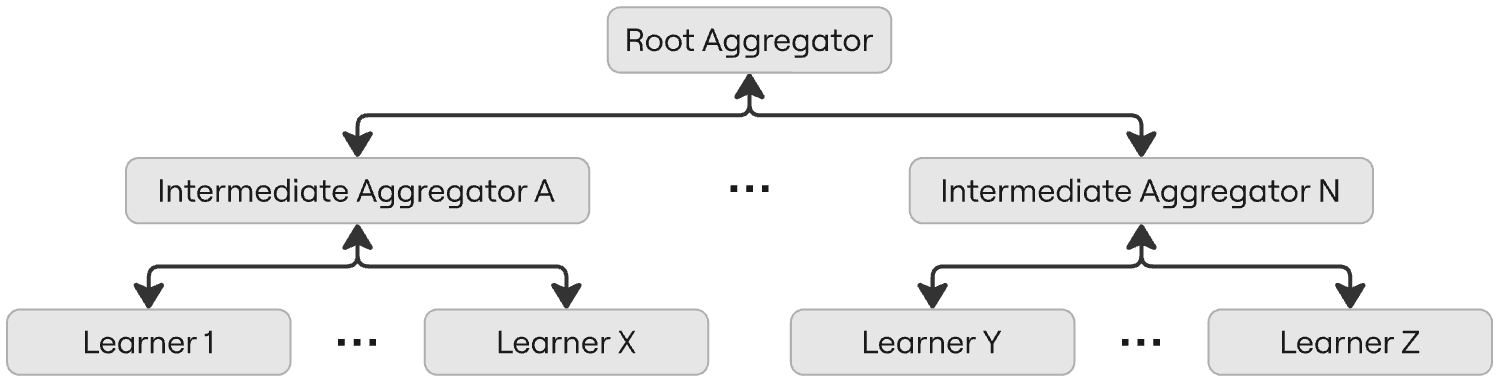
\includegraphics[width=\textwidth]{hfl_architecture.png}
    \caption{Hierarchical FL Architecture}
    \label{fig:hfl_architecture}
\end{figure}
Figure \ref{fig:hfl_architecture} depicts the hierarchical FL (HFL) architecture.
In HFL, the root aggregator delegates and distributes the aggregation task to intermediate aggregators.
HFL can have multiple layers of intermediate aggregators.
Each intermediate aggregator and its connected learners resemble an instance of classic FL.
After aggregating an intermediate model, the intermediate aggregators send their parameters upstream to the root aggregator.
The root combines the intermediate parameters into global ones and sends them downstream for further FL rounds.
HFL's structure requires changing the underlying FL architecture.

The proper design and implementation, and the assignment of learners to aggregators determine the success of one's FL setup.
For example, if too many learners are attached to a given aggregator, that aggregator becomes a bottleneck.
The intermediate aggregated model can be biased if too few learners are assigned.
Thus, the infrastructure resources and management costs become unjustified for the small number of learners.
A management overhead arises with more components, including handling fault tolerance, monitoring, synchronizing, and balancing.
Bad synchronization can amplify straggler problems.
Balancing refers to combining and harmonizing intermediate parameters to get a good global model.
These findings show that special FL architectures, such as HFL, require careful consideration and correct implementation.
\cite{book:fl,paper:decentralized_edge_intelligence_dynamic_resource_allocation_framework_hfl,hpfl_over_massive_mobile_edge_computing_networks}

The benefits of HFL are its dynamic scalability and load balancing.
One can easily add or remove intermediate aggregators and their connected learners.
Due to this distribution of load and aggregation, each aggregator, including the root, is less likely to face bottleneck issues.
One can combine HFL with CFL, where each intermediate aggregator is responsible for one or multiple clusters.
The downsides of HFL are communication and management overheads.
More components lead to more transmitted messages.
These messages all need to be secured and encrypted.
With more components and nodes, adversaries can take advantage of more possible backdoors.
HFL provides a powerful way to improve scalability for FL if done right.
\cite{
    paper:deploying_fl_in_hierarchical_edge_architecture,
    paper:hfl_with_momentum_acceleration_in_multi_tier_networks,
    paper:hfl_with_privacy,
    paper:decentralized_edge_intelligence_dynamic_resource_allocation_framework_hfl,
    book:fl,
    hpfl_over_massive_mobile_edge_computing_networks}


\subsubsection{Decentralized FL}
Decentralized FL does not require a central aggregator.
Instead, it operates on a peer-to-peer basis via a blockchain.
That way, the centralized communication bottleneck gets resolved.
The blockchain represents the global model.
Learners train in parallel.
Each locally trained update gets a version.
Based on this version, random clients are chosen for aggregation.
The results get appended to the blockchain, and the model version is incremented. \cite{book:fl}

\subsubsection{Asynchronous FL}
Asynchronous FL allows learners to train continuously and freely push their updates to the aggregator.
This method eliminates stragglers and dropout problems because a training round does not need to wait or handle outliers and timeouts.
A new issue of staleness arises when updates are merged into the global model that took a very long time to complete.
Such an update used a now outdated version of the global model.
As a result, the global model is partially reverted to an older state.
Asynchronous FL can be combined with other architectures. \cite{book:fl}

\subsection{FL Research}\label{subsection:fl_research}

\begin{figure}[h]
    \centering
    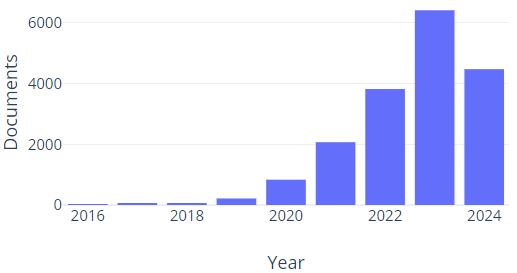
\includegraphics[width=0.8\textwidth]{fl_documents_research.png}
    \caption{Evolution of FL Publications}
    \label{fig:fl_documents_research}
\end{figure}

Figure \ref{fig:fl_documents_research} shows the exponential growth of FL documents since 2016.
(This data comes from searching for "federated learning" in article title, abstract, or keywords via Scopus \cite{scopus_homepage}.)
The idea for this graph is based on \cite{thesis:tum_fl_framework_comparison}.
Graph \ref{fig:fl_documents_research} uses a different query with the latest available data.

Before creating FLOps, we looked for research gaps in the fields of ML at the edge, specifically FL.
We have read and examined 47 papers in detail, with 26 papers focusing on FL. 
Additionally, we consulted several articles, joined and participated in discussion forums, and completed a couple of paid courses.
Discussing each paper in detail would heavily bloat this thesis.
This subsection presents key and meta-findings instead.
While working through the material, we created and incrementally updated a database in which we noted specific properties of each paper.
These properties include one or multiple categories in which the paper fits in.
Additional properties include the initial problems or challenges the authors tried to resolve, their contributions, results, limitations, and envisioned future work.
We also noted what ML or FL frameworks or libraries they claimed to use.

Table \ref{table:fl_research_table_1} depicts a subset of the analyzed FL papers.
It presents the documented contributions, limitations, and future work properties.
The remaining FL papers are available in Appendix \ref{appendix:fl_research}.
Note that we omit some of the 26 FL papers from these tables because we discuss them in greater detail throughout the background section.
These tables provide a good impression of the examined FL papers.
The following is a broad aggregated overview of a subset of these papers and their technical outcomes.
More precise individual insights of the examined paper are available in the mentioned tables.
Several papers \cite{paper:fl_inference_anytime_anywhere,paper:hfl_with_momentum_acceleration_in_multi_tier_networks,paper:model_pruning_for_edge_fl,paper:tackling_objective_inconsistency_problem_in_heterogeneous_fl} proposed novel learning methods that improve handling non-IID data, reduce resource usage, improve model quality, or train models quicker than previous methods.
Besides inventing or improving learning methods, others \cite{paper:refl_resource_efficient_fl,paper:edge_fl_via_mqtt_and_oma_lightweight_m2m,paper:fedat_high_performance_communication_efficient_fl_with_asynch_tiers} focus on new learner selection or aggregation algorithms to benefit the most from the available resources, especially from heterogeneous data.
Many works \cite{paper:edgefl_framework,paper:global_fl_platform_for_iot,paper:adaptive_exper_models_for_pfl} investigate the benefits and downsides of using different architectures for FL that lead to more efficient, performant, and scalable FL.
Other works \cite{paper:hfl_with_privacy, paper:cluster_based_secure_aggregation_for_fl,paper:efficient_privacy_preserving_ml_in_hierarchical_distributed_systems} focus on new privacy and security schemas or improve existing secure aggregation algorithms to reduce existing overheads and bottlenecks when using conventional protection.
A large portion of the examined works investigated and proved novel concepts to achieve a range of goals, from better privacy, scalability, and less overhead to better resource utilization.
Examples include \cite{paper:decentralized_edge_intelligence_dynamic_resource_allocation_framework_hfl,hpfl_over_massive_mobile_edge_computing_networks,paper:fl_toward_on_demand_client_deployment_at_edge}.
Patterns and trends can be extracted from these papers based on the documented properties.

\begin{figure}[p]
    \begin{changemargin}{-2cm}{0cm}
    \begin{tabular}{|c||m{0.4\paperwidth}|m{0.4\paperwidth}|}
        \hline
            ID & Contributions & Limitations \& Future Work \\
        \hline
            \cite{paper:refl_resource_efficient_fl}
            &
            A novel selection and staleness-aware aggregation strategy.
            Analysis of resource wastage and the impact of stragglers.
            A smart participation selection based on learner availability.
            &
            Privacy or security were not considered.
            Evaluations are based on classic datasets (MNIST, CIFAR-10), which do not reflect real non-IID data.
            Only homogeneous resources were assumed.
            Use of a simple linear regression model for availability prediction.
            More sophisticated alternatives exist.
            Factors such as battery level, bandwidth, and user preferences should also be considered for availability prediction.
        \\
        \hline
            \cite{paper:cluster_based_secure_aggregation_for_fl}
            &
            A novel cluster-based secure aggregation strategy for diverse nodes.
            Clustering based on processing score \& GPS information/latency leads to better throughput and reduces false-positive dropouts.
            A new additive sharing-based masking scheme that is robust against dropouts.
            &
            All participants are assumed to be honest.
            Malicious users were not considered.
            The aggregator might become a bottleneck, which can be resolved via HFL (with cluster heads).
            Image classification was the only evaluated ML task.
        \\
        \hline
            \cite{paper:privacy_preserving_deep_fl_for_coop_hierarchical_caching_in_fog_computing}
            &
            An FL caching scheme including novel algorithms and architecture.
            Utilization of an AI training model that considers user history.
            &
            A convergence analysis was not provided.
            For further security and privacy improvements, blockchain-empowered FL should be investigated.
        \\
        \hline
            \cite{paper:model_pretraining_and_initialization_for_fl}
            &
            Analysis of the impact of pre-training ML models for FL initialization compared to the common random approach.
            Findings show pre-trained model superiority.
            &
            It is challenging to get a pre-trained model if the necessary data is not available or private.
            Using pre-trained models can lead to biases.
            Only a specific (warm-start) initialization strategy was considered.
        \\
        \hline
            \cite{paper:decentralized_edge_intelligence_dynamic_resource_allocation_framework_hfl}
            &
            A novel incentive/resource-based allocation schema that utilizes game theory.
            Learners with more data are more valuable and they can compete for higher participation rewards.
            Multiple model owners compete for cluster heads with the most data.
            &
            The effects of social networks and their impact on worker's cluster selection decisions should be researched.
            Malicious workers were not considered.
        \\
        \hline
            \cite{paper:fedat_high_performance_communication_efficient_fl_with_asynch_tiers}
            &
            Synergy of asynchronous and synchronous FL via asynchronous tiers, which is able to handle stragglers.
            &
            The tiers all update the server individually.
            Further improvements are possible via HFL with intermediate cluster heads to do the aggregation.
            Additional security could be applied at these cluster heads.
        \\
        \hline
    \end{tabular}
    \captionof{table}{FL Papers considered for FLOps - Part I} 
    \label{table:fl_research_table_1}
\end{changemargin}

\end{figure}

\begin{figure}[p]
    \centering
    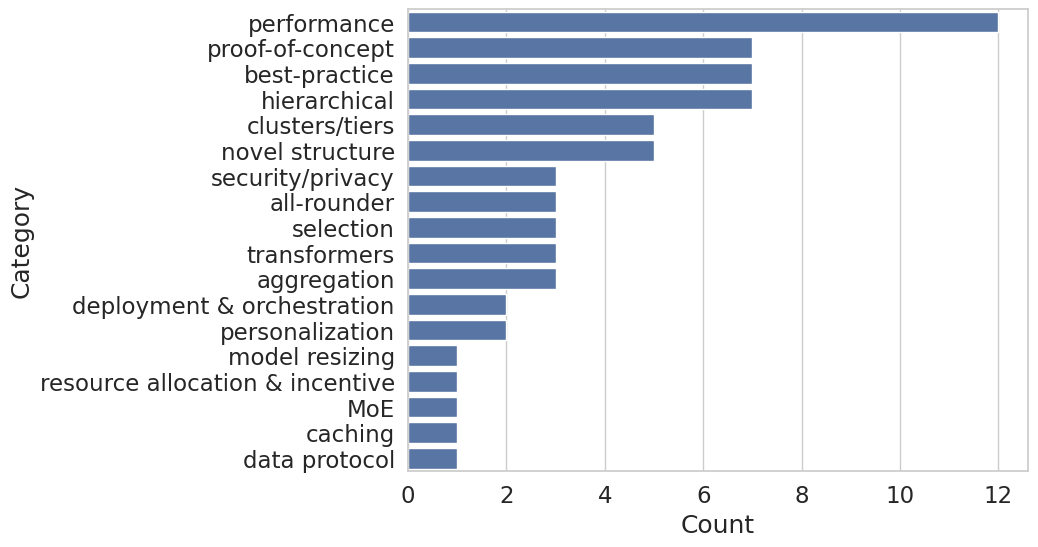
\includegraphics[width=1.0\textwidth]{fl_research_categories.png}
    \caption{FL Paper Categories}
    \label{fig:fl_research_categories}

    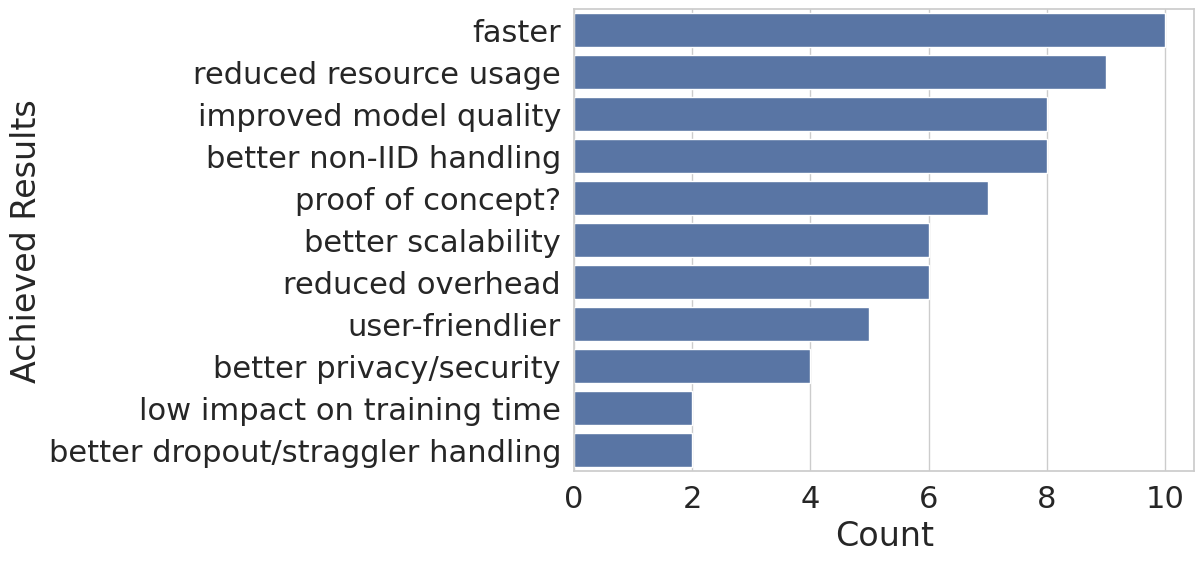
\includegraphics[width=0.9\textwidth]{fl_research_achieved_results.png}
    \caption{Achieved Results of FL Papers}
    \label{fig:fl_research_achieved_results}
\end{figure}

Patterns and trends help to better understand the research field of FL as a whole.
Figure \ref{fig:fl_research_categories} shows the different categories and their distribution.
Most examined papers focused on performance, trying new concepts, finding best practices, and exploring different FL architectures.
Only two papers focused on deployment and orchestration.

The achieved results match these categories.
Figure \ref{fig:fl_research_achieved_results} shows that these contributions lead to more efficient FL.
Improved aspects include speed, resource utilization, training results, and handling of heterogeneous data.
Additional insights about the research problems, contributions, limitations, and future work of the examined FL papers are available in the appendix \ref{appendix:fl_research}.

These documented properties might be biased, and the inspected sample size of papers is relatively small.
To improve confidence in these findings, we compare them with the total number of published works about FL.
Figure \ref{fig:fl_publications_compared} depicts how many works have been published in FL with specific keywords that match our custom categories.
We applied the same method to gather the data as for \ref{fig:fl_documents_research}.
The global results paint a similar picture as our samples.
The most popular topics in FL are related to privacy/security, performance, or algorithms.
Only a tiny portion of FL papers focus on usability, automation, orchestration, or other initial steps.

It seems that researchers assume others to already have working FL environments.
Furthermore, they seem to motivate their readers to optimize these setups based on their findings instead of replicating and configuring such an FL setup initially.
These tendencies are visible when inspecting the ML and FL frameworks and libraries the authors mentioned they used.
The following figure is again based on our examined papers.
Figure \ref{fig:fl_research_ml_and_fl_frameworks} shows that most authors did not explicitly state what ML framework or library they used for their work.
Many researchers used Pytorch and TensorFlow.
The figure also shows that FL researchers rarely mention what FL frameworks they use for their work.
It is much more common for authors to mention what ML framework they used than what FL framework they used.
Possible reasons for this might be that ML as a field is a lot older, more sophisticated, widespread, and established.
The same applies to ML frameworks.
On the other hand, FL is a very young subfield of ML research.
FL frameworks are still in their early stages.
FL researchers might be using FL frameworks.
However, due to the framework's immaturity, the researchers might not deem it important to explicitly point out that they used them.
Another possible explanation is that FL researchers are experts in FL and can set up and configure FL from the ground up.
Either way, this lack of transparency makes reproducing or extending their work challenging, if not infeasible.
These gaps in FL research motivated the creation of FLOps.

\begin{figure}[p]
    \centering
    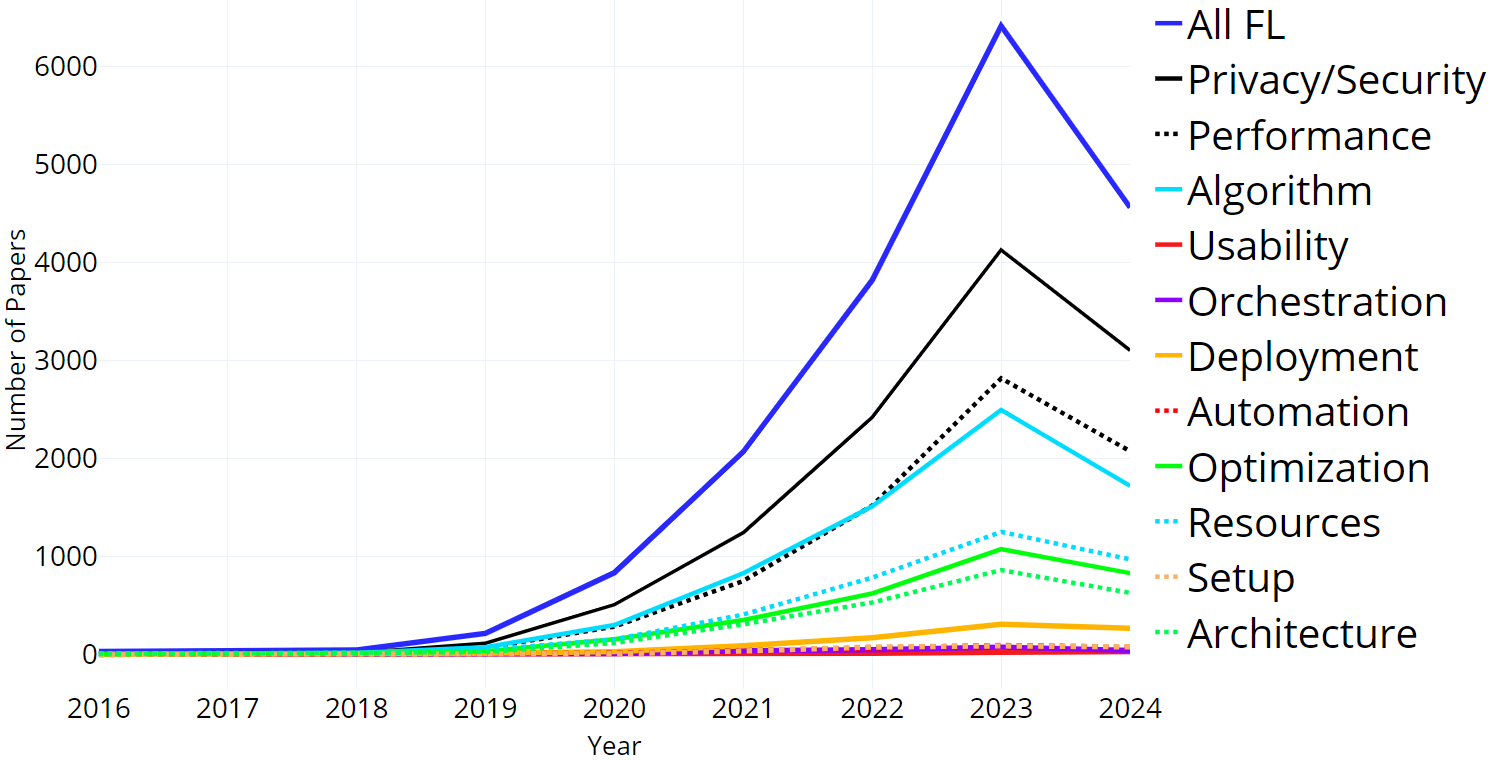
\includegraphics[width=1.0\textwidth]{fl_publications_compared.png}
    \caption{Evolution of FL Publications based on Keywords}
    \label{fig:fl_publications_compared}
    \vspace{2cm}
    \begin{adjustwidth}{-0.1\paperwidth}{-0.1\paperwidth}
        \centering
        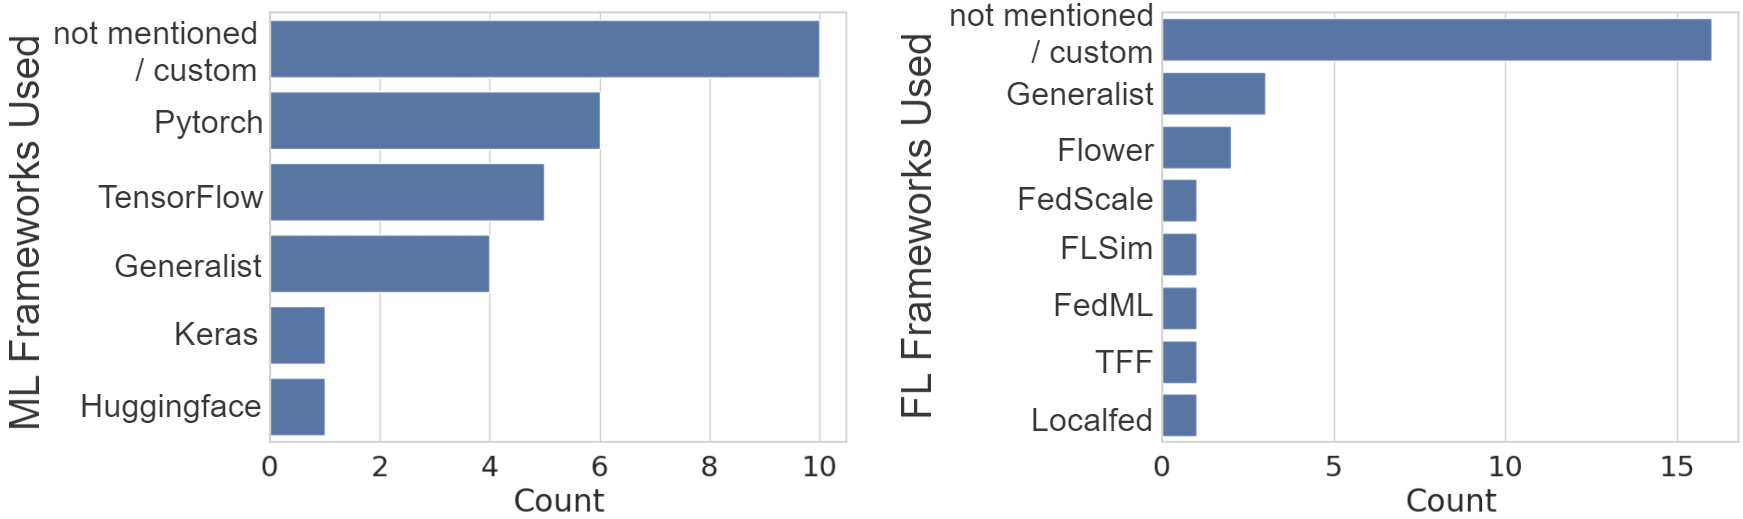
\includegraphics[width=0.8\paperwidth]{fl_research_ml_and_fl_frameworks.png}
        \caption{Distribution of mentioned ML and FL Frameworks in FL Papers}
        \label{fig:fl_research_ml_and_fl_frameworks}
    \end{adjustwidth}
\end{figure}

\pagebreak
\subsection{FL Frameworks \& Libraries}\label{subsection:fl_frameworks_and_libraries}

\begin{figure}[b]
    \begin{changemargin}{0cm}{0cm}
    \centering
    \begin{tabular}{|m{2.4cm}||c|c|c|c|c|c|}
        \hline
            \textbf{Framework} & \textbf{Version} & \textbf{Releases in 2024} & \textbf{Stars} & \textbf{Forks} & \textbf{Open Issues} \\
        \hline
            Pysyft \cite{fl_framework:pysyft} & 0.9.0 & 62 & 9.4k & 2k & 2
        \\
        \hline
            Tensorflow Federated \cite{fl_framework:tensorflow_federated} & 0.85.0 & 18 & 2.3k & 578 & 168
        \\
        \hline
            FedML \cite{fl_framework:fedml} & 0.8.9 & 0 & 4.1k & 776 & 118
        \\
        \hline
            Flower \cite{fl_framework:flower} & 1.10.0 & 4 & 4.7k & 815 & 284
        \\
        \hline
            OpenFL \cite{fl_framework:openfl} & 9.3.4 & 2 & 1.9k & 426 & 256
        \\
        \hline
    \end{tabular}
    \captionof{table}{Updated FL Framework Comparison} 
    \label{table:updated_fl_framework_comparison}
\end{changemargin}

\end{figure}

This subsection examines the current landscape of available FL frameworks.
The goal is to better comprehend why most researchers did not specify or use FL frameworks in the previous findings.
This discussion will be brief because Saidani already analyzed and evaluated FL frameworks in great detail in his master's thesis \cite{thesis:tum_fl_framework_comparison} from 2023.
He examined FL libraries, frameworks, and benchmarks.
Many FL tools exist for specific niche use cases and architectures \cite{thesis:tum_fl_framework_comparison}.
This finding contradicts the opinions of his questioned FL practitioners and experts.
They expected FL libraries and frameworks to focus on basic FL features, such as communication, aggregator-learner orchestration, security, and data aggregation.
Many libraries and frameworks, most of which were not production-ready, were still in an experimental research state \cite{thesis:tum_fl_framework_comparison}.

To reduce complexity, he focused on the five most promising open-source frameworks.
For a framework to be allegeable, it had to fulfill 2/3 of the following criteria.
It needed more than one thousand starts and 350 forks on GitHub.
The interviewed experts had to mention it.
The framework had to support all major operation systems.
Because FL is rapidly evolving, we updated his findings and expanded upon them.
We included the number of releases (including patches) in 2024 so far and the number of open issues in the repository.

Table \ref{table:updated_fl_framework_comparison} shows the updated FL Framework comparison (16.08.2024).
These FL frameworks are in active development. 
Only FedML has not been updated for several months now.

Saidani's main original contribution was a novel FL benchmarking suite called FMLB (Federated Machine Learning Benchmark).
Its goal was to evaluate and compare the mentioned FL frameworks efficiently.
His previous analysis and summary of existing frameworks were sound and helpful.
However, we are critical of his evaluation results, especially the poor performance of Flower.
We tried to replicate his experiments, but his provided code \cite{tum_fl_framework_thesis_github} lacks instructions on how to set up this benchmark application.
We simulated the experiments with the latest official flower version at the time and made sure to stick as closely as possible to the same experimental setup and configuration.
Our findings show very different results.
Flower manages to solve the experiment quickly and efficiently.
Our results match the verdicts of other works comparing FL frameworks, such as \cite{comparative_analysis_of_fl_frameworks} or \cite{comprehensive_study_fl_frameworks_degree_project}.
\cite{comparative_analysis_of_fl_frameworks} is the latest work that compares FL frameworks that we considered, and its verdict is that Flower outperforms all its competition.
FLOps uses Flower as its FL framework of choice.
\subsection{Flower} \label{subsection:flower}

Flower \cite{paper:flower} is a research-backed open-source FL framework.
One major target in Flower's paper was to narrow the gap between research and production.
It allows researchers to run high-performance FL simulations and rapidly transition to tangible production environments using the same tool.
Another focal point of its paper was scale and parallelization.

Flower is a sophisticated, feature-rich FL framework.
Flower's first release (0.10.0) was published in November 2020, and its first major release (1.0.0) was published in 2022 \cite{fl_framework:flower}.
Flower supports all major operating systems, containerization, and ML libraries.
It aims to be easily customizable and extendable via a programming language and ML framework agnostic design.
Flower strives to offer all popular FL features, such as support for different data types and distributions.
Further features include pre-implemented popular FL algorithms and vertical and horizontal data splitting support.
Flower supports traditional ML tasks, like regression or clustering, DNNs, LLMs, and security mechanisms, such as secure aggregation.
It enables the use of FL via CPUs or GPUs.
The default communication protocol is gRPC, which can be replaced.
Flower supports various FL variants, including PFL, edge computing, cross-silo, and cross-device.
It handles and implements core FL components but does not handle many other aspects, like deployment, orchestration, dependency management, or containerization.
Flower offers a mature set of FL simulation techniques.

Users can easily change and add functionality to the framework by interacting with flexible abstractions and interfaces.
The heart of Flower is its strategy concept.
The aggregator uses this strategy to manage the FL processes.
A strategy contains all necessary configurations, such as the FL algorithm and the minimum number of learners required for training or evaluation.
Users can pick from more than 30 existing strategies \cite{flower:strategies} or extend from basic strategies and develop their own behavior.
It does not have native out-of-the-box support for model pruning, advanced security/privacy techniques, CFL, HFL, MLOps, or orchestration.
Due to Flowers' flexible design, users can implement their custom features and strategies based on the available basic Flower components.

It is straightforward to set up Flower and start working with it.
Flower is directly available via Python's default package manager pip.
One has to define the server/aggregator, strategy, and clients/learners.
Users can implement the simplest case with a few dozen lines of Python code.
The crucial part is to configure the strategy and clients properly.
One needs to create a client class that extends from a Flower client and implement four essential methods that the framework will call during training.
These methods include a getter and setter for the model parameters and one method each for training/fitting and evaluating the model.
In conclusion, Flower provides a rapid and easy onboarding experience.

Flower has a modern, user-friendly, growing ecosystem.
A dedicated sub-project called Flower Datasets \cite{flower:datasets} is part of this ecosystem.
This project is still in its infancy (v0.3.0).
It allows users to pull HuggingFace \cite{hugging_face_homepage} datasets easily and split them into FL-optimized data fragments.
Users can configure how to split this data up.
Flower Datasets can turn standard non-federated homogeneous/IID datasets into challenging, federated, non-IID data, which is ideal for FL research and development.
This ecosystem includes a well-structured and rich homepage \cite{flower:homepage}, an extensive set of tutorials, guides, example projects \cite{flower:examples}, and documentation \cite{flower:homepage_docs, flower_docs} that ranges from beginner-friendly to advanced.
They have open monthly community events \cite{flower:monthly}, yearly summits \cite{flower:summit}, a blog \cite{flower:blog}, a discussion forum \cite{flower:forum}, a Slack space \cite{flower:slack}, and a YouTube channel \cite{flower:youtube}.


\section{Machine Learning Operations} \label{section:machine_learning_operations}

Investigating modern best practices is necessary to improve and benefit the field of FL.
Patterns emerged during the history of applying computer science to solve problems and develop solutions.
This includes various software engineering techniques and models.
Famous examples are the waterfall model or agile development, such as Scrum.
They all share the same goal of delivering high-quality, production-ready software.
Over the last decades, many contrasting and interconnected disciplines have emerged.
They must cooperate smoothly to develop, deliver, and operate modern software.
These tasks can be grouped into two broad categories: development and operation.


\subsection{DevOps}

The history of software development shows an evolution from static and isolated to dynamic and intertwined workflows.
Older methods like the waterfall model split up the development and operations tasks and involved individuals.
Software was first developed by one team and then operated by another.
There was a massive increase in modern requirements for flexibility and the ability to change.
Developmental and operational tasks now form an interconnected infinite loop.
For example, a company develops the first version of a software product in-house.
They build distributable software artifacts based on their source code for distribution among clients.
These artifacts might be container images or executable binaries.
They publish these artifacts to online registries and roll live services out in the cloud.
Users enjoy this product and request further features.
The loop starts anew.
The new features lead to unexpected bugs.
The loop starts again, and so on.
A software loop is only as fast as its slowest step.

In today's world, software development loops are rarely linear sets of steps.
Such loops are running in parallel at different stages several times per day.
This concurrency is especially noticeable in projects that divide software into multiple decoupled parts.
For example, in micro-service architectures, one service might be buggy and need fixing while another receives a feature update.
These dynamic and strong dependencies require developmental and operational tasks to work tightly together.
This coupling also applies to IT professionals who must cooperate and understand each other's areas well.
This combined effort has become its own broad disciple called DevOps.

The synergy between development and operations created new techniques, tools, and professions.
This combination includes various tasks such as building, deploying, testing, and monitoring.
Automation is one core activity in this connected discipline because repetitive manual labor is an inefficient and expensive bottleneck.
Prominent tools include Ansible and Gitlab-CI/CD.
DevOps is a very broad discipline without concrete borders.
Building artifacts or container images, orchestration, or knowledge sharing can all be considered part of DevOps.
This notion makes Git, Docker, and Kubernetes the primary tools in this field.

An essential concept in DevOps is CI/CD, which stands for continuous integration, continuous delivery, and deployment.
CI/CD focused on automating this software loop via custom pipelines.
A DevOps pipeline is comparable to an assembly line in a factory.
A software product needs to pass several connected stages with multiple steps.
These stages can include testing, building, releasing, and deployment.

DevOps as a term was first mentioned around 2009 \cite{paper:mlops}.
This field is still very active and rapidly evolving.
Unfortunately, many other disciplines are not taking inspiration from or taking advantage of DevOps.

\subsection{MLOps}

MLOps is a young discipline that uses many best practices and techniques from DevOps and applies them to ML.
Most DevOps techniques are applicable and beneficial for ML.
Further considerations and tooling are required to support specialized ML requirements.
ML differs from pure software development because it requires deep knowledge with different focal points, such as math and data science.
In addition, training, replicating, or understanding an ML model and its code requires extensive and usually untracked background knowledge.
This includes dependencies, environments, used training data, and whether the model is production-ready.
Additionally, a model only supports specific input and output values of certain types.
These unique requirements distinguish MLOps from conventional DevOps.

Inspecting the processes and challenges of a typical modern enterprise ML workflow demonstrates the need for MLOps.
An exemplary company wants to develop a new ML-based feature to satisfy customer needs.
Firstly, managers develop ideas for utilizing ML to solve these needs.
These ideas get evaluated, accessed, and distilled into formal requirements.
ML solutions require data for training and evaluation.
The company starts gathering suitable data by scouting for data sources and providers.
It collects and stores the found data in a custom data lake.
Data engineers can now start preparing this data for training.
Data preprocessing includes various steps, such as cleaning the data by removing outliers, wrong data samples, and undefined values.
Other steps transform the data to make it more suitable for training.
This includes applying normalization and standardization to slim down the feature space to reduce the curse of dimensionality.
Other steps involve data analysis and visualization to find insightful patterns and ensure that the available data is sound and useful.
These data preprocessing and data acquisition steps are an iterative process.
With this data, ML engineers can start designing ML models.

ML model training and deployment are resource- and time-consuming steps.
First model iterations are rarely ideal.
To reach optimality, models require multiple train and test cycles with different architectures, configurations of layers, and hyperparameters.
Just deploying a model is insufficient.
Models need to work as intended for expected and unexpected use cases.
The model performance can degrade over time.
This can occur if the model is allowed to change after the initial training and deployment phase.
Performance can also worsen for frozen models if circumstances change, such as the evolution of client needs and requests.
Therefore, deployed model instances and their inference serving quality need monitoring.
In case of bad performance, the model needs to be retrained or replaced with a better alternative.
Such an improved version needs to complete most of the discussed steps again before redeployment.
This workflow combines steps from business, management, data/ml/software engineering, and operations.
Usually, in larger organizations, each step is handled by a dedicated team of experts who require working closely together.
This exemplary workflow demonstrates that ML code and trained model alone cannot provide value in production environments.
Enterprise ML requires various supporting disciplines and techniques to be usable, including versioning and infrastructure management.
Due to these different iterative steps and stages, ML is a prime target for DevOps techniques.

MLOps is currently heavily underutilized, which slows down progress in ML enterprises.
Many trained ML models are not deployed on production systems to provide real value.
In 2020, only 14\% of trained enterprise ML models were deployed to production in less than a week \cite{algorithmia_state_of_enterprise_ml}.
Getting an ML model to run on production environments requires entirely different skill sets, which many pure ML professionals, researchers, and hobbyists lack.
Many individuals who perform ML lack training and industry experience as software engineers or developers.
They might be unaware of DevOps practices or that ML can greatly benefit from them.
To bring more awareness to MLOps, Kreuzberger et al. wrote a foundational paper \cite{paper:mlops} that provides an overview of MLOps and the current state of enterprise ML.
They propose the first attempts at definitions and best practices for MLOps, including recommended architectures, tools, and workflows.
They conclude that the field of ML is too fixated on academia and developing better ML models instead of optimizing tangible ML in production.
Their verdict mirrors and reinforces the findings from section \ref{subsection:fl_research} regarding similar gaps in FL research.
\subsection{MLflow}\label{subsection:mlflow}

MLflow \cite{mlflow:homepage} is a one-in-all open-source MLOps platform that enriches and unifies common ML tasks and provides automatic solutions for ML challenges.
Its first public version (0.2.0) was released in 2018.
Version 1.0.0 came out in 2019.
As of this writing, its latest version (2.15.1) was released in August 2024.
MLflow's repository \cite{mlflow:github} accumulated 18.2k stars, 4.1k forks, and 756 contributors.
Significant organizations, including Microsoft and Meta, use MLflow.
MLflow supports various popular ML tools and frameworks, such as Keras, Pytorch, HuggingFace, and more.
Furthermore, it is flexible for custom user extensions to support specialized functionality and tooling.
MLflow has a rich and active community and ecosystem.
This ecosystem includes detailed documentation \cite{mlflow:docs}, code examples \cite{mlflow:examples}, and places for discussion and receiving direct support (Slack).
A great resource besides the official ones to learn more about MLflow is this online course \cite{mlflow:udemy}.
MLflow helps users manage their ML workflow loops from conception to re-deployment.

MLflow divides its core features into multiple different interconnected components.
These components are rather conceptual groupings of functionalities than concrete isolated interfaces.
The following represents a major selection of critical components.
\vspace{5mm}
\newline
\textbf{Tracking}\newline
MLflow can track and log ML experiments to help users record and compare their ML results.
An experiment in MLflow is a set of runs.
Each run represents a specific execution of a piece of code.
A run can record various aspects of that execution, such as code version, metrics, or custom tags.
Users can customize what should be tracked and how often.
MLflow also offers automatic logging capabilities.
Popular targets for tracking include parameters ranging from hyperparameters to custom metaparameters.
The utilized code or training data can also be tracked, as well as metrics, such as accuracy and loss.
MLflow offers its tracking via various APIs, including Python, Java, and REST.
The tracking artifacts get recorded in a centralized place.
By default, these artifacts are recorded in a local directory.
These tracked records can also be stored and managed by a dedicated local or remote scalable tracking server.
That way, users can easily share the results they have tracked with others.
An MLflow tracking server comes with its own sophisticated and feature-rich web-based GUI.
This GUI allows users to inspect, compare, and manage their recorded findings easily.
MLflow tracking handles lightweight parameters, except for input data.
It does not track or record trained models (weights and biases).
\vspace{5mm}
\newline
\textbf{Models}\newline
MLflow can record and store ML models in uniform and popular formats.
Popular formats are called "flavors" in MLflow and include pickle formats, python functions, and ML framework-specific solutions.
Models can be stored together with exemplary input data, ML code, metadata, and a list of necessary dependencies for replication.
MLflow differentiates between storing lightweight parameters, meta-information, and models.
Model signatures can also be specified.
These signatures are similar to function signatures in programming.
They include the expected input and output types.
Other tools can utilize such signatures to automatically create the correct Python functions or REST APIs for a model.
Due to this standardized representation, many other tools can work with these models.
This uniformity also makes deploying these models more efficient.
MLflow allows users to deploy models to different environments via various ways, such as local inference servers (REST API), docker containers, and Kubernetes.
\vspace{5mm}
\newline
\textbf{Registry}\newline
MLflow's model registry is comparable to an interface or API that works with a subset of logged models.
It is not a dedicated standalone registry, unlike container image registries.
It does not host complete models.
This registry enables labeling and versioning for logged models.
Labeling includes specific information that tells users if the model is currently in development, review, or production-ready.
Not all logged models are part of the model registry.
Users can manually or automatically decide if and what models they want to add to the model registry.
This process is called registering a model.
Every registered model is also a logged model.
The benefit of this separation is that models in the registry are carefully selected and managed.
\vspace{5mm}
\newline
\textbf{Projects}\newline
Projects allow replicating the exact ML environment for development.
Unlike the tracked pieces of code from the tracking or model components, MLflow projects contain the entire codebase that was used to train a specific model.
Projects aim to uniformly package ML code for reproducibility and distribution.
The heart of an MLflow project is its MLproject file.
It contains all the necessary information regarding dependencies and environments to guarantee identical conditions.
This file can have multiple entry points, similar to a Docker file.
These entry points can be used for different use cases, including training or evaluation.
Other users can quickly start using such projects due to MLflow's project CLI commands.
A project's entry point can be called by the project CLI.
MLflow can also invoke a project as part of a dynamically built docker container.
The image gets built automatically via Docker after running the CLI command.
The CLI allows running projects that are local, remote, or stored in a git repository.
MLflow projects have a lot of potential, but they are not yet capable of fully handling robust automatic containerization and dependency management.
They work fine if run directly on a host machine that supports Docker.
Most orchestrators expect images and deploy containers.
It is not yet possible to orchestrate and deploy MLflow projects directly instead of using manually configured images.
Issues arise when wrapping an MLflow project into a generic image and then internally calling its CLI to build and run the corresponding image.
MLflow uses Docker directly, which is, in most cases, not possible inside a containerized environment.
This limitation is represented in the official MLflow examples \cite{mlflow:docker_example}.
In this example, all necessary dependencies are explicitly mentioned and installed in a custom Dockerfile that needs to be built manually to run the ML experiments.
This emphasizes that MLflow projects cannot be automatically turned into standalone container images yet.
\vspace{5mm}
\newline
MLflow stores its artifacts in two different data stores.
The default does not use any dedicated local or remote storage components.
Instead, everything gets stored locally.
All lightweight metadata, including metrics, tags, and results, are stored in the backend store.
A backend store can be a database, a file server, or a cloud service.
Heavy artifacts like trained models are kept in the artifact store.
Registered models utilize both stores.
Their metadata, such as versions and hyperparameters, are kept in the backend store.
Their corresponding trained model is located in the artifact store.

MLflow supports many optional components that can be arranged in various architectures.
In the simplest case, everything is stored and located on the local machine, with no need for a dedicated tracking server or data stores.
More sophisticated structures support shared and distributed workflows and workloads.
The mentioned components can be gradually added or removed.
Therefore, MLflow allows flexible and custom solutions.
For example, the artifact store, backend store, and tracking server can all be deployed on different machines and environments.
This separation of concerns enables improved scalability and reduces singular points of failure.
The tracking server can function as a proxy and bridge between machines that perform the ML experiments and the data stores.
This approach enables centralized security and access control, which simplifies client interactions.

MLflow lacks native support for FL.
It does not explicitly mention or support FL.
However, FL can profit from MLflow due to its modular design, that can be customized and applied to FL specific components and environments.
For that reason, FLOps is using MLflow.


\section{Orchestration}

Modern orchestration and containerization techniques have been rapidly evolving for the last decade.
To avoid issues due to different environments and dependencies, containers arose as a lightweight alternative to heavier virtual machines.
The most popular containerization software, Docker, was released in 2013.
Multiple individual containers quickly got grouped together to separate concerns and allow decoupled workloads.
These container groups became especially useful and popular with the rise of micro-service architectures.
Handling various containers at the same time is challenging.
Techniques such as Docker Compose made this easier.
However, dynamically scaling and handling failing containers was still difficult.
These dynamic swarms of containers needed additional management tooling for orchestration.
Kubernetes, the most prominent orchestrator to date, was released in 2014.
Since then many new endevours formed to unify and streamline future developents in the field.
Examples include the Open Container Initiative \cite{open_container_initiative} or the Moby Project \cite{moby_project}.
Many different alternatives and competitors to Docker and Kubernetes have developed over the years.

\subsection{ML Containerization \& Orchestration}

Performing ML in containers is an effective approach.
FLOps aims to automate and orchestrate FL workloads on distributed heterogeneous machines.
It is crucial to confirm that doing FL/ML via orchestrated containers is viable.
In addition, FL processes should not suffer from bottlenecks and problems due to running inside containers.
In 2017, Xu et al. \cite{paper:dl_via_docker} evaluated deep learning (DL) tool performance in docker containers.
They analyzed CPU, GPU, and I/O utilizations.
They found that DL works equally well in containers as running it directly on the host machines.

Containerized ML is widely used today.
In 2022, Openja et al. \cite{paper:ml_practices_on_docker} analyzed more than 400 different open-source ML-based projects that use docker containers.
These projects used containers for various tasks.
A popular application of containerization technologies in ML is to streamline and improve deployment efforts.
This work demonstrates that containers are used in all ML-related tasks nowadays.

Orchestration efforts are optional for classic ML but essential for FL.
As discussed in \ref{section:federated_learning}, classic centralized ML can be trained on a single powerful machine.
FL, especially Cross-Device edge FL, can involve massive dynamic numbers of devices.
Managing all these components is challenging.
Training an ML model requires more than just the ML code and model.
The device performing the training needs to support the necessary environment and dependency requirements.
The setup and configuration of devices is a limiting and error-prone task.
To avoid potential issues and to allow as many devices to participate as possible, FL should use containers. 


\subsection{Oakestra}

FLOps primarily focuses on enabling practical FL on real machines.
The main target group for cross-device FL is heterogeneous edge devices.
Kubernetes is not designed for the edge but for homogeneous, resource-rich cloud environments, whereas Oakestra is designed for the edge and outperforms Kubernetes there \cite{paper:oakestra_usenix}.

Oakestra is a hierarchical, open-source orchestrator for edge computing.
It has a lightweight and flexible code base.
It features many novel techniques, such as semantic overlay networking for efficient service communication.

\begin{figure}[!ht]
    % \begin{adjustwidth}{-\oddsidemargin-1in}{-\rightmargin}
    \begin{adjustwidth}{-0.1\paperwidth}{-0.1\paperwidth}
        \centering
        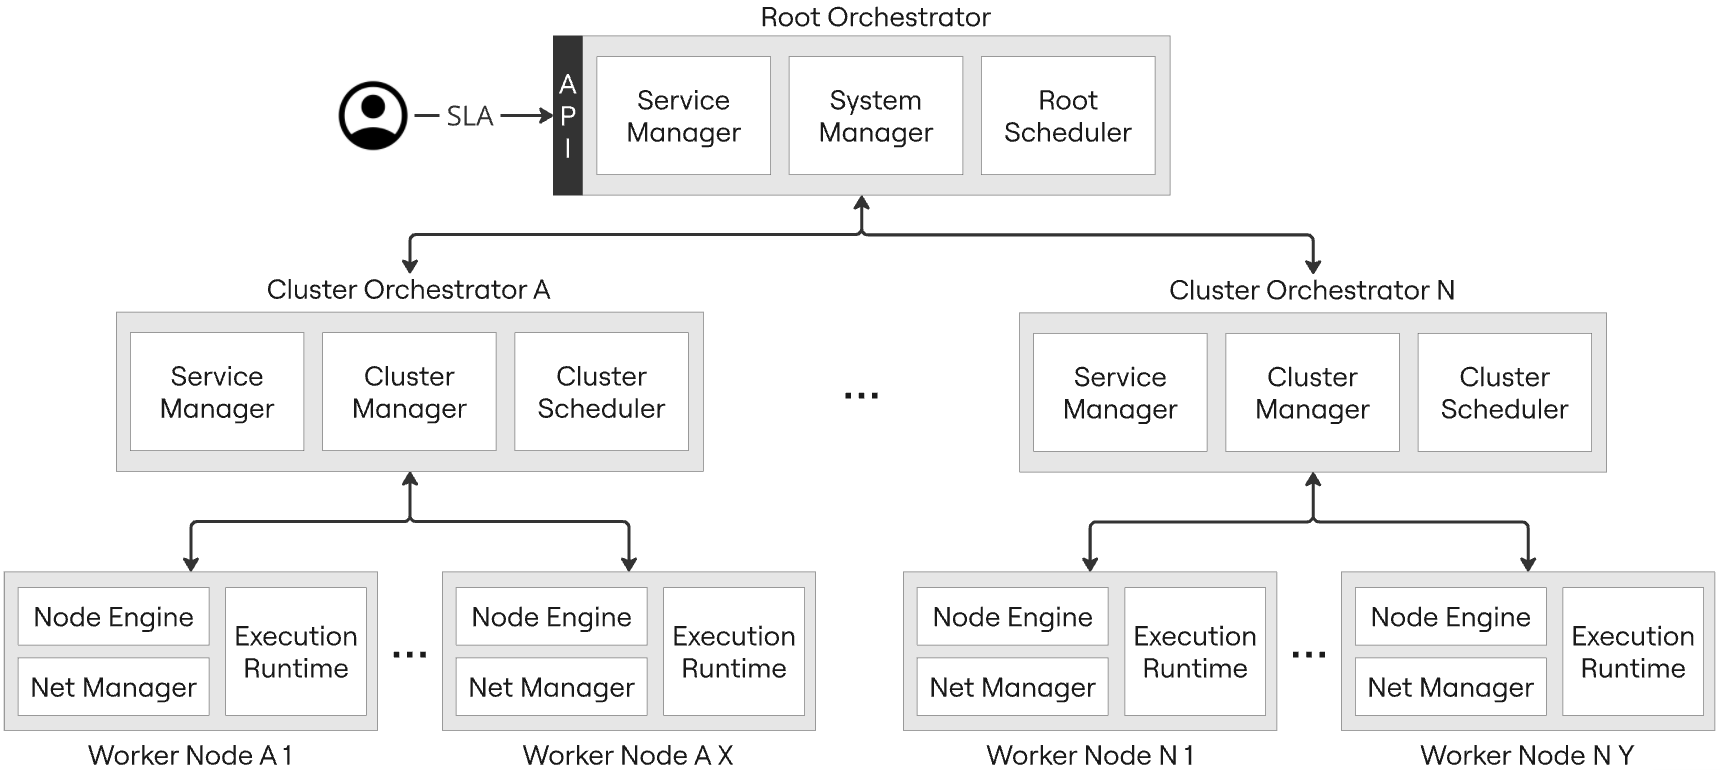
\includegraphics[width=0.9\paperwidth]{oakestra_simple_architecture.png}
        \caption{Simplified Oakestra Architecture}
        \label{fig:simple_oakestra_architecture}
    \end{adjustwidth}
\end{figure}

Figure \ref{fig:simple_oakestra_architecture} shows a simplified architecture of Oakestra.
This unique federated three-tiered structure allows for scalable delegate task scheduling and execution.
Instead of a single control plane, as in Kubernetes, Oakestra distributes its control among the root and cluster orchestrators.
Oakestra specializes in handling resource-constrained, heterogeneous devices that are spread across various geographical areas.
Different infrastructure providers can have their own isolated cluster and cluster orchestrator.
Cluster orchestrators can only access detailed information about workers from their own cluster.
The metrics they share with the root are distilled and no longer contain sensitive individual metadata.
This is an ideal environment for FL because this layout supports privacy on a structural level.
FLOps uses Oakestra to orchestrate its components.

\pagebreak


\section{Related Work}

Only two previous works \cite{paper:fl_toward_on_demand_client_deployment_at_edge, paper:global_fl_platform_for_iot} mentioned in subsection \ref{subsection:fl_research} resemble FLOps.
Both also noticed the lack of research regarding dynamically deploying ML and FL capabilities via containers.
They use different technologies and offer different functionality compared to FLOps.
They focus on other aspects and do not incorporate MLOps tools, automatic image builds, or automatic deployment of trained model inference servers.

In 2023, Chahoud et al. \cite{paper:fl_toward_on_demand_client_deployment_at_edge} proposed a three-layered FL architecture running on Kubernetes.
The first layer is the server or service provider that handles managerial responsibilities.
It serves container images to voluntary devices and maintains secure connections to other layers.
The server aggregates the global model using a threshold to handle stragglers and missing or failed updates.
Together with the mini-servers, it determines which nodes should form a cluster.
It handles service deployments and client selection after receiving requests from mini-servers.
Various components are part of the server.
An oracle engine determines the required ML type and builds the client base model.
A Kubeadm environment initializer turns devices into mini-servers based on availability.
An orchestrator manager dynamically administers the second layer mini-servers which handle clusters and surveil devices.
They deploy containers and add workers to clusters.
Mini-servers distribute management tasks and workloads among themselves and away from the server while gathering metrics and informing the server via aggregated updates.
Mini-servers and the "root" server resemble Oakestra's root and cluster orchestrators.

In 2022, Safri et al. \cite{paper:global_fl_platform_for_iot} developed a prototype to improve FL on IoT devices.
This work focuses on enterprise IoT and enables distributed ML model deployment, federated task orchestration, and system state and model performance monitoring.
This three-layered architecture resembles the one from \cite{paper:fl_toward_on_demand_client_deployment_at_edge} and Oakestra.
Their root server/orchestrator acts as an FL aggregator and dynamically configures and deploys local orchestrators via an API.
Their local orchestrator is different from cluster orchestrators or mini-servers.
IoT devices are usually incapable of handling common ML training due to their limited resources.
Their work acknowledges this and uses the IoT devices only as data providers but not as learners.
Therefore, their work performs classic FL instead of HFL.
Local orchestrators are learners in their architecture.
They need to be in proximity to IoT devices to receive their data.
Additionally, they provide customizable data preprocessing and evaluation code to be injected via the API.
Their work offers additional tooling, such as a custom compressor, which reduces the size of large files and monitoring.
Monitoring agents are deployed on the local and global orchestrators that measure resources and CO2.
A custom GUI presents these metrics.

Open challenges and future work include more efficient and secure selection algorithms.
To optimize FL results via data heterogeneity, more sophisticated (metrics-based) logic is required to select learners for training.
Chahoud et al. wanted to investigate the mini-server selection to minimize potential security hazards.

There are apparent similarities between their works and FLOps/Oakestra.
All three focus on making FL easy to use and do not focus on optimizing models or algorithms.
Containerization technologies enable on-the-fly dynamic deployment and setup of FL components on unprepared devices.
All provide prepared container images via public registries.
Safri et al. also want to provide a one-in-all solution to perform FL on tangible devices.
They want to automate setup, dependency management, configuration, and metric gathering.
Additionally, they want to improve comprehension and observability by providing a GUI.

Their works differ from FLOps in multiple ways besides FLOps' more extensive set of features.
They use different orchestrators, FL frameworks (augmented FedML), and image registries.
Oakestra is a dedicated orchestrator, while their work's components are auxiliaries with fewer features and less mature architectures.
FLOps supports classic and hierarchical FL.
\cite{paper:fl_toward_on_demand_client_deployment_at_edge} only support HFL, and \cite{paper:global_fl_platform_for_iot} only support classic FL.
They used a single hardcoded dataset and ML model for evaluation.
Their works do not offer different scenarios or utilize dedicated MLOps features and techniques.
FLOps allows users to build and train various custom ML code.
Chahoud et al. focus on 6G and the actual real-world movement of people, whereas FLOps is more general and feature-rich.
Safri et al.'s paper is very short and thus lacks details and readability.
It has no open-sourced code to inspect and replicate its implementation.
FLOps has this thesis documenting it in great detail and is fully open source.
Their works implement most components by themselves from the ground up, such as orchestration and FL.
FLOps utilizes and combines existing sophisticated solutions to offer higher-quality features and performance.
For example, \cite{paper:global_fl_platform_for_iot}'s GUI is a simple Grafana dashboard with fewer features and is read-only.
FLOps utilizes MLflow to provide a sophisticated graphical suite of MLOps tools and functionalities.
